\documentclass[11pt,a4paper]{article}

\usepackage[T1]{fontenc}
\usepackage[utf8]{inputenc}
\usepackage{lmodern}
\usepackage{microtype}
\usepackage[a4paper,margin=1in]{geometry}
\usepackage{setspace}
\usepackage{graphicx}
\usepackage{float}
\usepackage{booktabs}
\usepackage{array}
\usepackage{multirow}
\usepackage{xcolor}
\usepackage{hyperref}
\usepackage{listings}
\usepackage{enumitem}
\usepackage{titlesec}
\usepackage{fancyhdr}
\usepackage{caption}
\usepackage{tikz}
\usetikzlibrary{positioning,arrows.meta}

\onehalfspacing
\renewcommand{\arraystretch}{1.2}

\definecolor{darkblue}{RGB}{20,50,120}
\definecolor{lightgray}{RGB}{245,245,245}

\hypersetup{
colorlinks=true,
linkcolor=darkblue,
urlcolor=darkblue,
citecolor=darkblue
}

\lstset{
backgroundcolor=\color{lightgray},
basicstyle=\ttfamily\small,
breaklines=true,
frame=single,
numbers=left,
numberstyle=\tiny
}

\titleformat{\section}{\Large\bfseries}{\thesection}{1em}{}
\titleformat{\subsection}{\large\bfseries}{\thesubsection}{1em}{}

\pagestyle{fancy}
\fancyhf{}
\fancyhead[L]{Legal RAG}
\fancyhead[R]{Project Proposal}
\fancyfoot[C]{\thepage}

\begin{document}

\begin{titlepage}
\centering
\vspace*{2cm}

{\Huge\bfseries Legal RAG\par}
\vspace{0.4cm}
{\Large Legal Assistant for Indian Case Law\par}

\vspace{2cm}
{\Large Project Proposal\par}

\vspace{2cm}

Dheeraj Murthy\\
Mathew Joseph\\
Ayush Tiwari

\vfill

\textbf{International Institute of Information Technology Bangalore}

\vspace{0.5cm}
\today
\end{titlepage}

\pagenumbering{roman}

\begin{abstract}
India's legal ecosystem produces massive volumes of judgments that are
difficult to search manually. Existing legal research tools are expensive
and not optimized for Indian legal language. We present a
Retrieval-Augmented Generation system that ingests 26,000+ Supreme Court
judgment PDFs, indexes them as dense vector embeddings in PostgreSQL with
pgvector, and answers legal queries using a two-stage retrieval pipeline
followed by local LLM inference. The architecture combines BGE dense
embeddings, cross-encoder reranking, and Qwen2.5-7B-Instruct to deliver
grounded, citation-anchored answers without external API calls.
\end{abstract}

\vspace{0.3cm}
\noindent
\fbox{\parbox{\textwidth}{
\textbf{Project Snapshot}
\begin{itemize}[noitemsep]
\item Corpus: 26,000+ Supreme Court Judgments
\item Vector Store: PostgreSQL + pgvector
\item Embeddings: BGE Base v1.5
\item Reranker: MiniLM Cross Encoder
\item LLM: Qwen2.5-7B-Instruct
\item Deployment: Docker Compose
\end{itemize}
}}

\tableofcontents
\newpage
\pagenumbering{arabic}

\section{Problem Statement}

India's legal ecosystem produces massive volumes of judgments, appeals, and
legal commentary. However:

\begin{itemize}[noitemsep]
    \item Legal texts are long, complex, and difficult to search manually.
    \item Lawyers and students spend hours reading case law without tooling
        support.
    \item Existing legal research tools (Westlaw, SCC Online) are expensive
        and not optimized for Indian legal language and citation patterns.
\end{itemize}

There is a clear need for an open, accessible NLP system that understands
Indian legal terminology, retrieves relevant precedents with high recall,
and generates grounded answers with verifiable citations.

\section{Background}

This project began as a Project Elective under Prof.\ Tulika at IIIT
Bangalore, focused on building NLP systems for the Indian legal scene.
Over the previous semester, we developed a 2-stage RAG pipeline
accumulating data from over 50,000 Indian Supreme Court judgments
spanning 75+ years, using a Qwen Instruct model to create a chatbot
that understands Indian law and answers queries relevant to the Indian
Penal Code and jurisdiction.

As part of our research and market analysis, we conducted surveys and
interviews with students, professors, and working alumni from reputed
National Law Universities including NLSIU Bangalore and NUSRL Ranchi.
The full survey outcomes are available in the accompanying file
\texttt{AI Legal Assistant -- User Assessment Survey(1-217).xlsx}.

\section{Vision and Objectives}

\subsection{Vision}

Build a production-ready NLP system tailored to Indian legal language
that enables fast semantic search, grounded question-answering,
summarization, and insights over court judgments.

\textbf{Target users:} Lawyers, law students, legal researchers, LegalTech
startups, and citizens checking case context.

\subsection{Core Objectives}

\begin{itemize}[noitemsep]
    \item Build a searchable case-law knowledge base from 26,000+ Supreme
        Court judgment PDFs.
    \item Deliver grounded Q/A over legal queries with verifiable case
        citations.
    \item Provide high-quality summaries of judgments with quoted passages.
    \item Facilitate petition generation from case context and legal principles.
    \item Create a secure, scalable web API and chat UI.
\end{itemize}

\subsection{Out of Scope}

\begin{itemize}[noitemsep]
    \item Predicting case outcomes.
    \item Replacing qualified legal professionals.
\end{itemize}

\section{Datasets}

The system uses three datasets:

\paragraph{1. LLM Fine Tuning Dataset of Indian Legal Texts}
Curated question-answer pairs from the Indian Penal Code (IPC),
Criminal Procedure Code (CRPC), and the Indian Constitution.
Used for instruction-tuning evaluation and prompt development.\\
\url{https://www.kaggle.com/datasets/akshatgupta7/llm-fine-tuning-dataset-of-indian-legal-texts}

\paragraph{2. Indian Supreme Court Judgments}
A CSV index of judgments extracted from the government API, including
PDFs and metadata (court, case number, date, language). Updated weekly.
Metadata includes a language column; some entries span multiple years.\\
\url{https://www.kaggle.com/datasets/vangap/indian-supreme-court-judgments}

\paragraph{3. Legal Dataset: SC Judgments India (1950--2024)}
26,000+ PDFs covering approximately 98\% of Supreme Court judgments
available on Indian Kanoon. Primary corpus for the vector knowledge
base, spanning 75+ years of Indian legal history. Each file represents
an official judgment delivered by the Supreme Court of India.\\
\url{https://www.kaggle.com/datasets/adarshsingh0903/legal-dataset-sc-judgments-india-19502024}

\section{System Architecture}

\subsection{Two-Stage Retrieval Pipeline}

The system follows a four-step pipeline:

\begin{enumerate}[noitemsep]
    \item \textbf{Stage 1 -- High-Recall Retrieval:} User query is embedded
        with \texttt{BAAI/bge-base-en-v1.5} (768-dimensional dense vectors).
        PostgreSQL/pgvector performs cosine similarity search using an HNSW
        index. Returns 30 candidate chunks at a similarity threshold of 0.2.
    \item \textbf{Stage 2 -- Cross-Encoder Reranking:} A cross-encoder
        (\texttt{cross-encoder/ms-marco-MiniLM-L-6-v2}) scores each
        (query, chunk) pair. The top 8 chunks are selected for context.
    \item \textbf{Generation:} Selected chunks are formatted into a Qwen
        chat-template prompt with strict grounding instructions. The LLM
        runs with \texttt{temperature=0.2, do\_sample=False} (greedy
        decoding) for deterministic output grounded only in the provided
        context.
    \item \textbf{Post-Processing:} Citations are extracted from response
        text, confidence scores are computed from embedding similarity and
        lexical overlap, and quality metrics are reported per query.
\end{enumerate}

\begin{figure}[H]
\centering
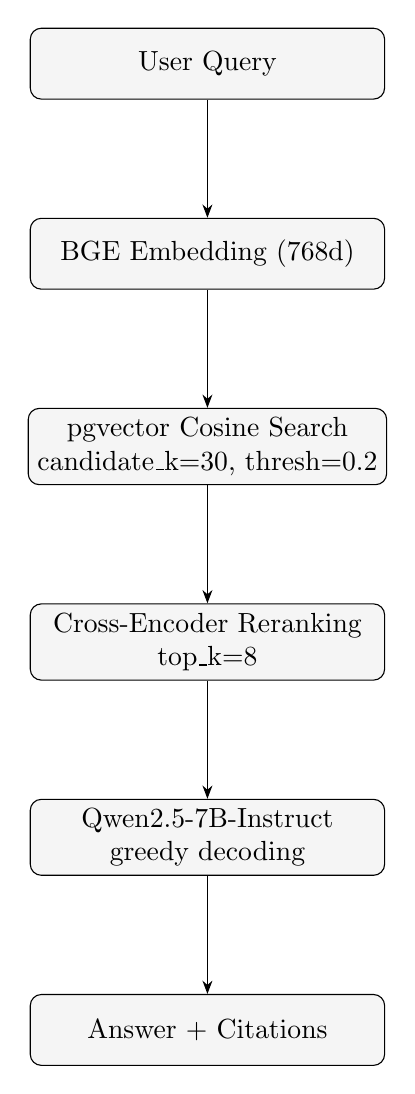
\begin{tikzpicture}[
node distance=1.5cm,
box/.style={draw,rounded corners,minimum width=4.5cm,minimum height=0.9cm,align=center,fill=lightgray},
>=Stealth
]
\node[box] (u) {User Query};
\node[box,below=of u] (e) {BGE Embedding (768d)};
\node[box,below=of e] (r) {pgvector Cosine Search\\candidate\_k=30, thresh=0.2};
\node[box,below=of r] (x) {Cross-Encoder Reranking\\top\_k=8};
\node[box,below=of x] (l) {Qwen2.5-7B-Instruct\\greedy decoding};
\node[box,below=of l] (a) {Answer + Citations};

\draw[->] (u)--(e);
\draw[->] (e)--(r);
\draw[->] (r)--(x);
\draw[->] (x)--(l);
\draw[->] (l)--(a);
\end{tikzpicture}
\caption{End-to-End RAG Pipeline}
\end{figure}

\subsection{System Components}

The FastAPI server orchestrates five modular components:

\begin{itemize}[noitemsep]
    \item \textbf{Retriever} (\texttt{retriever.py}): Connects to PostgreSQL,
        generates query embeddings via sentence-transformers, executes
        cosine similarity search with HNSW index.
    \item \textbf{Reranker} (\texttt{reranker.py}): Loads a CrossEncoder
        model, scores candidate chunks, returns top-N by relevance.
    \item \textbf{Prompt Builder} (\texttt{prompt\_builder.py}): Formats
        retrieved chunks into a Qwen-instruct template with a strict
        system prompt: ``Answer ONLY using the provided context.''
    \item \textbf{LLM Inference} (\texttt{llm\_inference.py}): Loads
        Qwen2.5-7B-Instruct-1M via HuggingFace transformers with
        \texttt{device\_map="auto"} and \texttt{torch.float16}.
    \item \textbf{Post-Processor} (\texttt{post\_processor.py}): Cleans
        responses, extracts citations, computes confidence scores, and
        formats output.
\end{itemize}

\section{Tech Stack}

\begin{table}[H]
\centering
\begin{tabular}{ll}
\toprule
\textbf{Layer} & \textbf{Technology} \\
\midrule
Backend Framework & Python 3.11, FastAPI, Uvicorn \\
Large Language Model & Qwen/Qwen2.5-7B-Instruct-1M \\
Embeddings Model & BAAI/bge-base-en-v1.5 (768d) \\
Cross-Encoder Reranker & cross-encoder/ms-marco-MiniLM-L-6-v2 \\
Vector Database & PostgreSQL 16 + pgvector (HNSW index) \\
PDF Ingestion & pdftotext (poppler-utils), PyPDF2 \\
Optical Character Recognition & Tesseract + pytesseract + pdf2image \\
Frontend & Next.js (chatbot-ui) + bare HTML/JS fallback \\
Containerization & Docker Compose (postgres, api, frontend) \\
Hardware & GPU with $\sim$16 GB VRAM (NVIDIA) \\
\bottomrule
\end{tabular}
\caption{Technology Stack}
\end{table}

\section{Database Schema}

Three tables form the core schema. Judgments are split into sections
(facts, issues, arguments, ratio, judgment) and each chunk is embedded
as a 768-dimensional vector for cosine similarity search.

\begin{lstlisting}[language=SQL]
CREATE TABLE judgments (
    id SERIAL PRIMARY KEY,
    petitioner TEXT,
    respondent TEXT,
    court TEXT,
    date_of_judgment DATE,
    bench TEXT[],
    citations JSONB,
    judgment_text TEXT
);

CREATE TABLE judgment_chunks (
    chunk_id SERIAL PRIMARY KEY,
    judgment_id INTEGER REFERENCES judgments(id)
        ON DELETE CASCADE,
    section TEXT CHECK (section IN (
        'facts', 'issues', 'arguments',
        'ratio', 'judgment'
    )),
    content TEXT
);

CREATE TABLE judgment_embeddings (
    chunk_id INTEGER PRIMARY KEY
        REFERENCES judgment_chunks(chunk_id)
        ON DELETE CASCADE,
    embedding vector(768) NOT NULL
);

CREATE INDEX judgment_embedding_hnsw_idx
    ON judgment_embeddings
    USING hnsw (embedding vector_cosine_ops);
\end{lstlisting}

\section{Software Requirements}

\subsection{Functional Requirements}

\begin{itemize}[noitemsep]
    \item Answer legal questions with grounded case citations:
        \begin{itemize}[noitemsep]
            \item Search judgments by semantic similarity.
            \item Refuse or warn when answer is unsupported by retrieved
                context.
            \item Include ``not legal advice'' disclaimer.
        \end{itemize}
    \item Show authoritative supporting cases: court, year, paragraph ID.
    \item Display quoted passages from judgments, not just references.
    \item Preserve traceability through chunk-to-judgment mapping.
    \item Handle conversation: follow-up questions via chat mode,
        clarification when no results found.
\end{itemize}

\subsection{Non-Functional Requirements}

\begin{itemize}[noitemsep]
    \item \textbf{Performance:} Retrieval in $\sim$200\,ms, generation in
        $\sim$2--4\,s. Scales with corpus size via HNSW index.
    \item \textbf{Accuracy:} Strict context-only prompting prevents
        hallucination. Confidence scoring combines embedding similarity
        and lexical overlap.
    \item \textbf{Security:} Self-hosted GPU inference. No external API
        calls for legal data. Zero user data logged externally.
    \item \textbf{Maintainability:} Modular pipeline design.
        Per-query metrics and debug information available.
    \item \textbf{UX:} Consistent response format across CLI, API, and
        web UI.
\end{itemize}

\section{Deployment}

\subsection{Docker Compose (Recommended)}

\begin{lstlisting}[language=bash]
docker-compose -f deploy/docker/docker-compose.yml up -d
\end{lstlisting}

\begin{table}[H]
\centering
\begin{tabular}{lll}
\toprule
\textbf{Service} & \textbf{Port} & \textbf{Description} \\
\midrule
postgres & 5432 & PostgreSQL 16 + pgvector \\
api & 8000 & FastAPI backend (Uvicorn) \\
frontend & 3000 & Next.js chat interface \\
\bottomrule
\end{tabular}
\end{table}

\subsection{Manual Setup}

\begin{lstlisting}[language=bash]
# 1. Initialize database
bash deploy/db_setup/init_db.sh

# 2. Ingest judgment PDFs
python database/ingest.py --input /path/to/pdfs

# 3. Start API server
cd rag_model && python api.py

# 4. Query via CLI
cd rag_model && python main.py \
    --query "principles of natural justice?"
\end{lstlisting}

\subsection{API Endpoints}

\begin{table}[H]
\centering
\begin{tabular}{lll}
\toprule
\textbf{Endpoint} & \textbf{Method} & \textbf{Description} \\
\midrule
\texttt{/query} & POST & Single grounded query \\
\texttt{/chat} & POST & Multi-turn chat with memory \\
\texttt{/chat/clear} & POST & Clear conversation history \\
\texttt{/chat/history} & GET & Retrieve chat history \\
\texttt{/document} & POST & OCR + query on PDF/image \\
\texttt{/retrieval-test} & POST & Debug retrieval (no LLM) \\
\texttt{/status} & GET & System configuration \\
\bottomrule
\end{tabular}
\end{table}

\subsection{CLI Usage}

\begin{lstlisting}[language=bash]
# Single query
python main.py --query "What are the principles of natural justice?"

# Interactive mode
python main.py --interactive

# Chat with memory
python main.py --chat

# Retrieval-only (no GPU needed)
python main.py --retrieval-test
\end{lstlisting}

\section{Evaluation Methodology}

\begin{itemize}[noitemsep]
    \item \textbf{Recall@K}: Proportion of relevant chunks retrieved
        in the top-K candidates for each query.
    \item \textbf{Mean Reciprocal Rank (MRR)}: Average reciprocal rank
        of the first relevant result across test queries.
    \item \textbf{Citation Accuracy}: Fraction of generated citations
        that map to valid, retrieved chunks in the context.
    \item \textbf{Response Groundedness}: Lexical overlap between the
        generated answer and the provided context chunks.
    \item \textbf{End-to-End Latency}: Total time from query submission
        to response delivery, measured across the pipeline stages.
\end{itemize}

\section{Project Status}

\begin{table}[H]
\centering
\begin{tabular}{lll}
\toprule
\textbf{Component} & \textbf{Status} & \textbf{Completion} \\
\midrule
Core RAG Pipeline & Complete & 100\% \\
Database Layer & Complete & 100\% \\
FastAPI Backend & Complete & 100\% \\
Next.js Frontend & Complete & 100\% \\
Docker Deployment & Complete & 100\% \\
OCR Support & Complete & 100\% \\
High Court Scraper & In Progress & 60\% \\
CI/CD Pipeline & Planned & 0\% \\
Production Monitoring & Planned & 0\% \\
\bottomrule
\end{tabular}
\caption{Project Status Overview}
\end{table}

\section{Future Work}

\begin{itemize}[noitemsep]
    \item \textbf{Petition Generation}: Build templates and LLM-guided
        drafting workflows for legal petitions grounded in retrieved
        case law.
    \item \textbf{Hybrid Retrieval}: Combine dense vector search with
        sparse keyword retrieval (BM25) for improved recall.
    \item \textbf{Multilingual Support}: Extend to handle Indian regional
        language judgments (Hindi, Kannada, Tamil, etc.).
    \item \textbf{High Court Integration}: Expand beyond Supreme Court to
        include Karnataka, Delhi, Bombay, and other High Courts.
    \item \textbf{Citation Graph Search}: Enable traversal of citation
        networks between judgments.
    \item \textbf{Fine-tuned Legal Models}: Instruction-tune a smaller
        LLM specifically on Indian legal question-answer pairs.
    \item \textbf{Automated Evaluation}: Build a benchmark suite with
        curated legal queries and ground-truth citations.
\end{itemize}

\section*{Disclaimer}
This system is a research tool and does not constitute legal advice.

\end{document}
